\documentclass[dvipsnames]{beamer}
\usepackage[utf8]{inputenc}
\usepackage{listings}
\usepackage{comment}
\usepackage{soul}
%\usepackage{ulem}
\usepackage{subfig}
\setul{}{1pt}
\usepackage[oldenum, olditem]{paralist}
%allow even smaller text
\newcommand\tinytiny{\fontsize{4pt}{3}\selectfont}

\makeatletter
\let\old@lstKV@SwitchCases\lstKV@SwitchCases
\def\lstKV@SwitchCases#1#2#3{}
\makeatother
\usepackage{lstlinebgrd}
\makeatletter
\let\lstKV@SwitchCases\old@lstKV@SwitchCases

\lst@Key{numbers}{none}{%
    \def\lst@PlaceNumber{\lst@linebgrd}%
    \lstKV@SwitchCases{#1}%
    {none:\\%
     left:\def\lst@PlaceNumber{\llap{\normalfont
                \lst@numberstyle{\thelstnumber}\kern\lst@numbersep}\lst@linebgrd}\\%
     right:\def\lst@PlaceNumber{\rlap{\normalfont
                \kern\linewidth \kern\lst@numbersep
                \lst@numberstyle{\thelstnumber}}\lst@linebgrd}%
    }{\PackageError{Listings}{Numbers #1 unknown}\@ehc}}
\makeatother


\graphicspath{{logos/}}

\usepackage{tikz}
\graphicspath{{4_0/figures/}}
%disclaimer for Sandia. uncomment and the whole blob goes away @ b80c116300122
\def\sandid{SANDXXXX PE}

% \title{Performance Portability with Kokkos}
\title{Kokkos 4.3 Release Briefing}

%BAD misuse of author field
\author{New Capabilities}


\usetheme{kokkos}

\newif\ifshort
\newif\ifmedium
\newif\iffull
\newif\ifnotoverview

\newcommand{\TutorialDirectory}{\texttt{Intro-Full}}
\newcommand{\ExerciseDirectory}[1]{\texttt{Exercises/#1/}}
\newcommand{\TutorialClone}{\texttt{Kokkos/kokkos-tutorials/\TutorialDirectory}}

\definecolor{darkgreen}{rgb}{0.0, 0.5, 0.0}
\definecolor{darkred}{rgb}{0.8, 0.0, 0.0}
\definecolor{orange}{rgb}{0.8, 0.33, 0.0}
\definecolor{purple}{rgb}{0.60, 0.20, 0.80}
\colorlet{bodyColor}{blue!20}
\colorlet{patternColor}{orange!30}
\colorlet{policyColor}{green!30}

% http://tex.stackexchange.com/questions/144448/color-a-text-line-in-a-code-lstlisting
\lstnewenvironment{code}[1][]%
{
  %with txfonts: OT1/txr/m/n/10
  %with default fonts: OT1/cmr/m/n/10
  %\fontfamily{cmr}\selectfont
  %\showthe\font
   \noindent
   \minipage{\linewidth}
   %\vspace{0.5\baselineskip}
   \lstset{mathescape, escapeinside={<@}{@>},
moredelim=**[is][{\btHL[fill=patternColor]}]{@pattern}{@pattern},
moredelim=**[is][{\btHL[fill=red!30]}]{@warning}{@warning},
moredelim=**[is][{\btHL[fill=policyColor]}]{@policy}{@policy},
moredelim=**[is][{\btHL[fill=bodyColor]}]{@body}{@body},
moredelim=**[is][{\btHL[fill=red!30]}]{@warning}{@warning},
moredelim=**[is][\color{black}]{@black}{@black},
moredelim=**[is][\color{blue}]{@blue}{@blue},
moredelim=**[is][\bf]{@bold}{@bold},
moredelim=**[is][\it]{@italic}{@italic},
moredelim=**[is][\color{boldblue}\bf]{@boldblue}{@boldblue},
moredelim=**[is][\color{red}]{@red}{@red},
moredelim=**[is][\color{green}]{@green}{@green},
moredelim=**[is][\color{gray}]{@gray}{@gray},
moredelim=**[is][\color{darkgreen}]{@darkgreen}{@darkgreen},
moredelim=**[is][\color{darkred}]{@darkred}{@darkred},
moredelim=**[is][\color{orange}]{@orange}{@orange},
moredelim=**[is][\color{purple}]{@purple}{@purple},
keywords={},
#1}
}
{
  \endminipage
  %\vspace{1.0\baselineskip}
}

\makeatletter
\newif\ifATOlinebackground
\lst@Key{linebackground}{\tiny}{\def\ATOlinebackground{#1}\global\ATOlinebackgroundtrue}
\makeatother

\lstnewenvironment{shell}[1][]{%
  \global\ATOlinebackgroundfalse
  \lstset{language=sh,%
    showstringspaces=false,
    aboveskip=0pt,
    frame=none,
    numbers=none,
    belowskip=2pt,
    breaklines=true,
    #1,
    }
  %\ifATOlinebackground
  \lstset{linebackgroundcolor={
    \ATOlinebackground
  }}
  %\fi
  }{}

\lstnewenvironment{cmake}[1][]{%
  \global\ATOlinebackgroundfalse
  \lstset{language=sh,%
    showstringspaces=false,
    aboveskip=0pt,
    frame=none,
    numbers=none,
    belowskip=2pt,
    breaklines=true,
    #1,
    }
  %\ifATOlinebackground
  \lstset{linebackgroundcolor={
    \ATOlinebackground
  }}
  %\fi
  }{}

\newcommand{\inlinecode}[1]{{\lstset{basicstyle=\ttfamily,keywordstyle={},showstringspaces=false}\lstinline$#1$}}
\newcommand{\inlineshell}[1]{{\lstset{basicstyle=\ttfamily,keywordstyle={},showstringspaces=false}\lstinline$#1$}}

\setbeamercolor{block title}{fg=white, bg=SandiaLightBlue}
\setbeamercolor{block body}{bg=lightgray}
\setbeamercolor{block title alerted}{fg=white, bg=SandiaRed}
\setbeamercolor{block body alerted}{bg=lightgray}



%\usepackage[texcoord,grid,gridunit=mm,gridcolor=red!10,subgridcolor=green!10]{eso-pic}
\usepackage[absolute,overlay]{textpos}





% http://tex.stackexchange.com/questions/8851/how-can-i-highlight-some-lines-from-source-code

\usepackage{pgf, pgffor}
\usepackage{listings}
\usepackage{lstlinebgrd} % see http://www.ctan.org/pkg/lstaddons

\makeatletter
%%%%%%%%%%%%%%%%%%%%%%%%%%%%%%%%%%%%%%%%%%%%%%%%%%%%%%%%%%%%%%%%%%%%%%%%%%%%%%
%
% \btIfInRange{number}{range list}{TRUE}{FALSE}
%
% Test in int number <number> is element of a (comma separated) list of ranges
% (such as: {1,3-5,7,10-12,14}) and processes <TRUE> or <FALSE> respectively

\newcount\bt@rangea
\newcount\bt@rangeb

\newcommand\btIfInRange[2]{%
    \global\let\bt@inrange\@secondoftwo%
    \edef\bt@rangelist{#2}%
    \foreach \range in \bt@rangelist {%
        \afterassignment\bt@getrangeb%
        \bt@rangea=0\range\relax%
        \pgfmathtruncatemacro\result{ ( #1 >= \bt@rangea) && (#1 <= \bt@rangeb) }%
        \ifnum\result=1\relax%
            \breakforeach%
            \global\let\bt@inrange\@firstoftwo%
        \fi%
    }%
    \bt@inrange%
}
\newcommand\bt@getrangeb{%
    \@ifnextchar\relax%
        {\bt@rangeb=\bt@rangea}%
        {\@getrangeb}%
}
\def\@getrangeb-#1\relax{%
    \ifx\relax#1\relax%
        \bt@rangeb=100000%   \maxdimen is too large for pgfmath
    \else%
        \bt@rangeb=#1\relax%
    \fi%
}

%%%%%%%%%%%%%%%%%%%%%%%%%%%%%%%%%%%%%%%%%%%%%%%%%%%%%%%%%%%%%%%%%%%%%%%%%%%%%%
%
% \btLstHL<overlay spec>{range list}
%
% TODO BUG: \btLstHL commands can not yet be accumulated if more than one overlay spec match.
%
\newcommand<>{\btLstHL}[2]{%
  \only#3{\btIfInRange{\value{lstnumber}}{#1}{\color{#2}\def\lst@linebgrdcmd{\color@block}}{\def\lst@linebgrdcmd####1####2####3{}}}%
}%
\makeatother






% http://tex.stackexchange.com/questions/15237/highlight-text-in-code-listing-while-also-keeping-syntax-highlighting
%\usepackage[T1]{fontenc}
%\usepackage{listings,xcolor,beramono}
\usepackage{tikz}

\makeatletter
\newenvironment{btHighlight}[1][]
{\begingroup\tikzset{bt@Highlight@par/.style={#1}}\begin{lrbox}{\@tempboxa}}
{\end{lrbox}\bt@HL@box[bt@Highlight@par]{\@tempboxa}\endgroup}

\newcommand\btHL[1][]{%
  \begin{btHighlight}[#1]\bgroup\aftergroup\bt@HL@endenv%
}
\def\bt@HL@endenv{%
  \end{btHighlight}%
  \egroup
}
\newcommand{\bt@HL@box}[2][]{%
  \tikz[#1]{%
    \pgfpathrectangle{\pgfpoint{1pt}{0pt}}{\pgfpoint{\wd #2}{\ht #2}}%
    \pgfusepath{use as bounding box}%
    \node[anchor=base west, fill=orange!30,outer sep=0pt,inner xsep=1pt, inner ysep=0pt, rounded corners=3pt, minimum height=\ht\strutbox+1pt,#1]{\raisebox{1pt}{\strut}\strut\usebox{#2}};
  }%
}
\makeatother



\usetikzlibrary{calc}
\usepackage{xparse}%  For \NewDocumentCommand

% tikzmark command, for shading over items
\newcommand{\tikzmark}[1]{\tikz[overlay,remember picture] \node (#1) {};}

\makeatletter
\NewDocumentCommand{\DrawBox}{s O{}}{%
    \tikz[overlay,remember picture]{
    \IfBooleanTF{#1}{%
        \coordinate (RightPoint) at ($(left |- right)+(\linewidth-\labelsep-\labelwidth,0.0)$);
    }{%
        \coordinate (RightPoint) at (right.east);
    }%
    \draw[red,#2]
      ($(left)+(-0.2em,0.9em)$) rectangle
      ($(RightPoint)+(0.2em,-0.3em)$);}
}

\NewDocumentCommand{\DrawBoxWide}{s O{}}{%
    \tikz[overlay,remember picture]{
    \IfBooleanTF{#1}{%
        \coordinate (RightPoint) at ($(left |- right)+(\linewidth-\labelsep-\labelwidth,0.0)$);
    }{%
        \coordinate (RightPoint) at (right.east);
    }%
    \draw[red,#2]
      ($(left)+(-\labelwidth,0.9em)$) rectangle
      ($(RightPoint)+(0.2em,-0.3em)$);}
}

\NewDocumentCommand{\DrawBoxWideBlack}{s O{}}{%
    \tikz[overlay,remember picture]{
    \IfBooleanTF{#1}{%
        \coordinate (RightPoint) at ($(left |- right)+(\linewidth-\labelsep-\labelwidth,0.0)$);
    }{%
        \coordinate (RightPoint) at (right.east);
    }%
    \draw[black,#2]
      ($(left)+(-\labelwidth,0.9em)$) rectangle
      ($(RightPoint)+(0.2em,-0.3em)$);}
}
\makeatother

\usetikzlibrary{positioning}

\usetikzlibrary{shapes}

\hypersetup{
    colorlinks=true,
    linkcolor=blue,
    filecolor=magenta,
    urlcolor=cyan,
}



\shorttrue
\mediumfalse
\fullfalse

\begin{document}

\begin{frame}
        \titlepage
\end{frame}


\begin{frame}[fragile]{Outline}

\textbf{4.3 Release Highlights}

    \begin{itemize}
      \item{Organizational}
      \item{Backend updates}
      \item{Build system updates}
      \item{\texttt{Kokkos::sort\_by\_key}}
      \item{Miscellaneous}
      \item{Deprecations and other breaking changes}
    \end{itemize}

\end{frame}

\begin{frame}{Find More}

\textbf{Online Resources}:

\begin{itemize}
        \item \url{https://github.com/kokkos}:
                \begin{itemize}
                        \item Primary Kokkos GitHub Organization
                \end{itemize}
        \item \url{https://github.com/kokkos/kokkos-tutorials/wiki/Kokkos-Lecture-Series}:
                \begin{itemize}
			\item{Slides, recording and Q\&A for the Full Lectures}
                \end{itemize}
        \item \url{https://kokkos.github.io/kokkos-core-wiki}:
                \begin{itemize}
                        \item Wiki including API reference
                \end{itemize}
        \item \url{https://kokkosteam.slack.com}:
                \begin{itemize}
                        \item Slack channel for Kokkos.
                        \item Please join: fastest way to get your questions answered.
                        \item Can whitelist domains, or invite individual people.
                \end{itemize}
\end{itemize}

\end{frame}

\begin{frame}[fragile]{Kokkos Usage}
  \textbf{Would like to strengthen community bonds and discoverability}

\vspace{10pt}
\textit{List of Applications and Libraries}
\begin{itemize}
\item Add your app to \url{https://github.com/kokkos/kokkos/issues/1950}
\item We are planning to add that to a Kokkos website.
\item Helps people discover each other when working on similar things.
\end{itemize}

\vspace{10pt}
\textit{GitHub Topics}
\begin{itemize}
\item Use \textit{kokkos} tag on your repos.
\item If you click on the topic you get a list of all projects on github with that topic.
\end{itemize}

\end{frame}

\begin{frame}[fragile]{Kokkos Topic}
  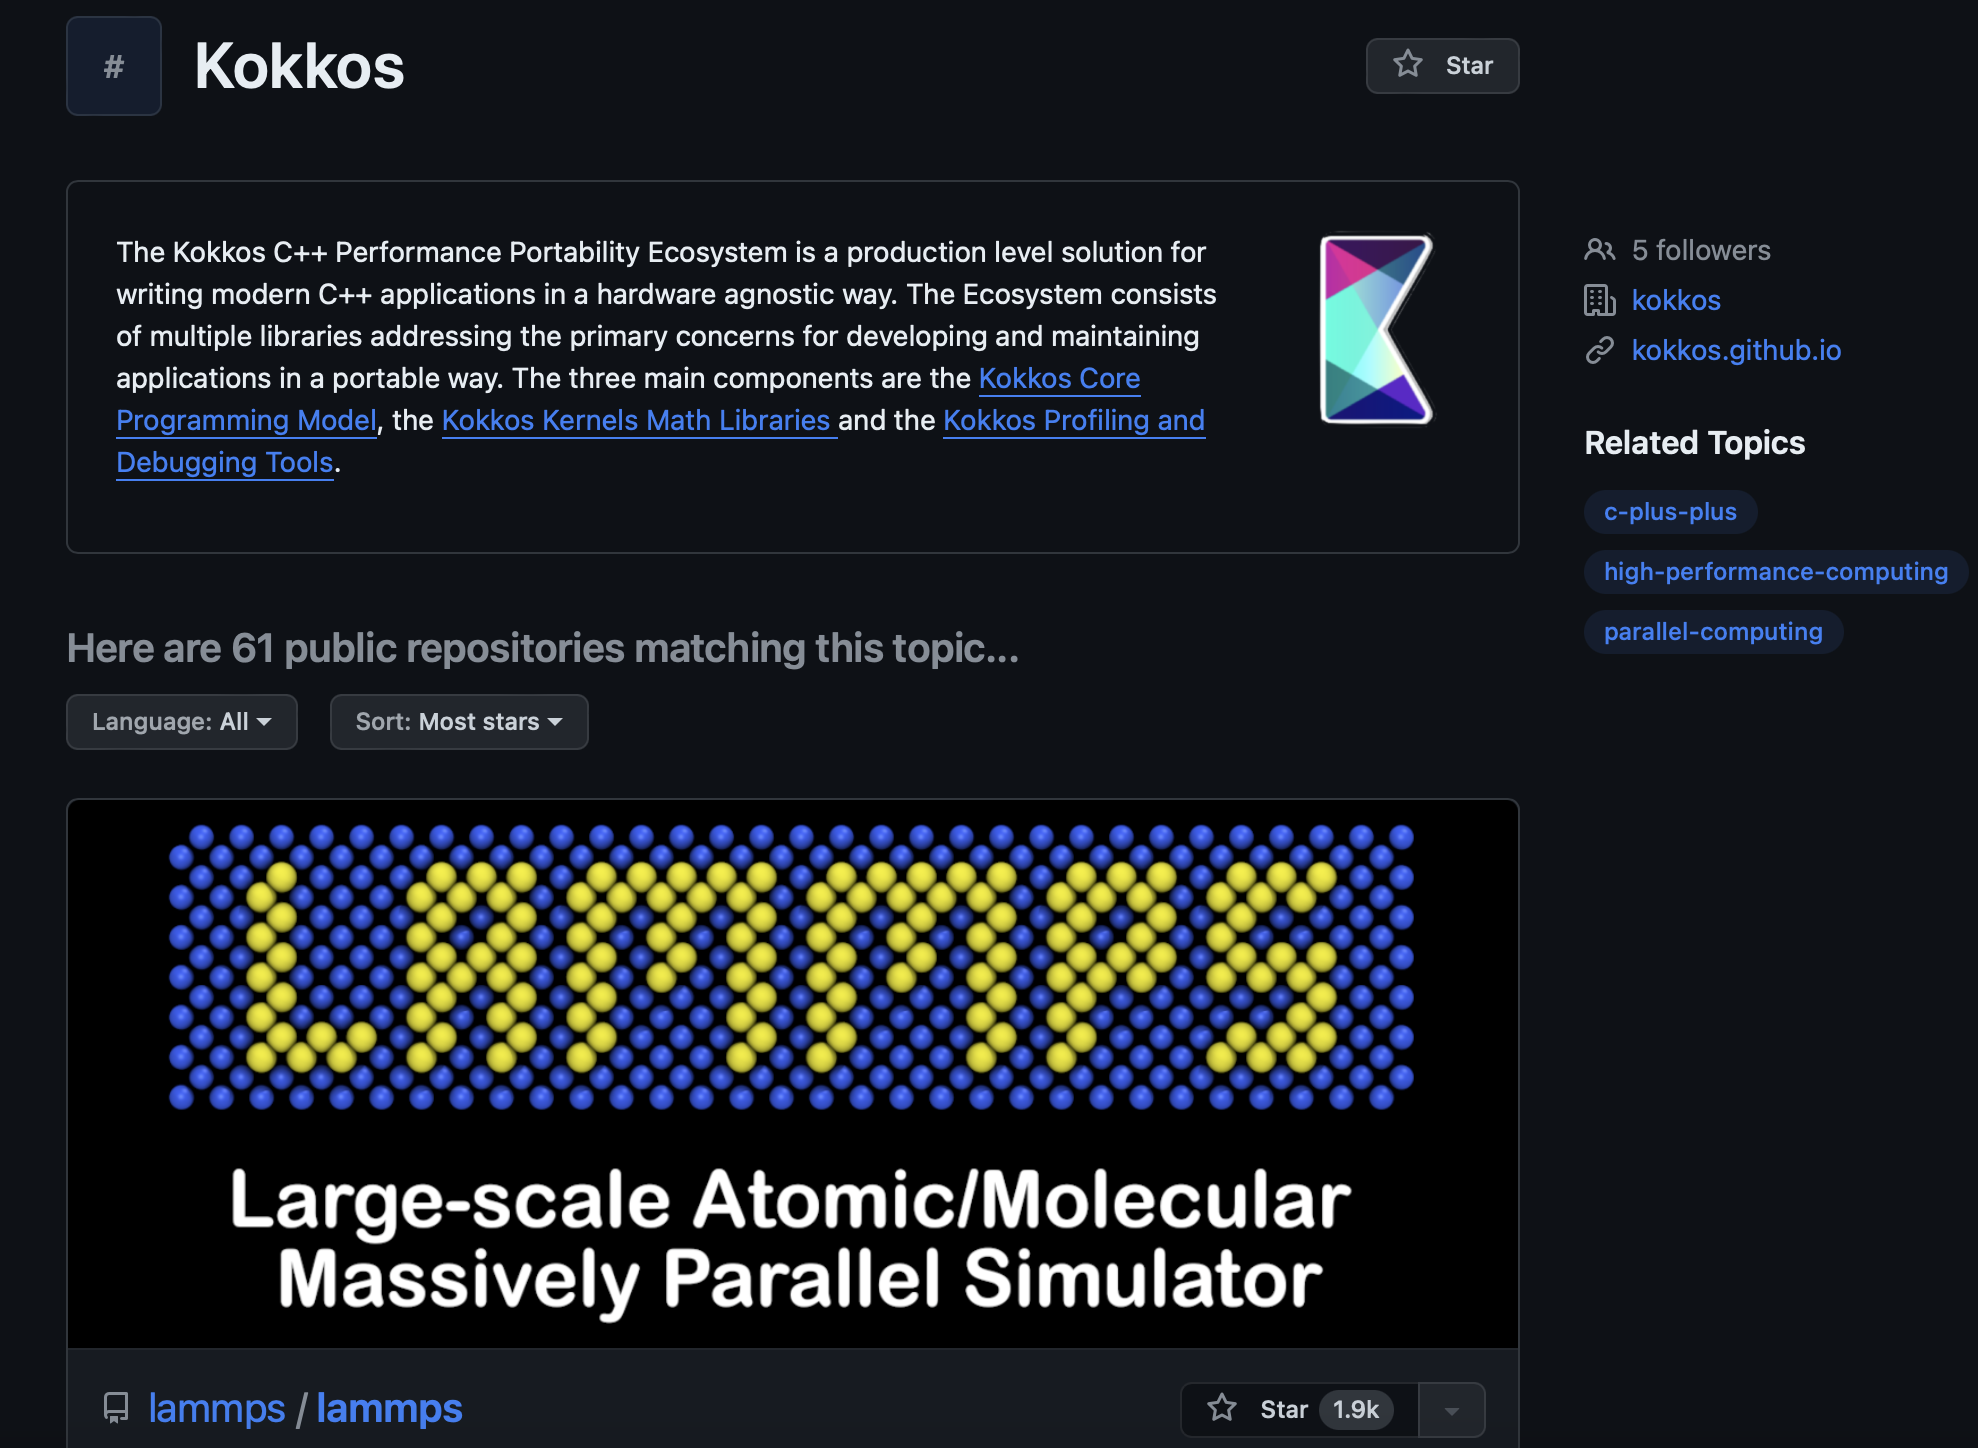
\includegraphics[width=0.9\textwidth]{4_3/kokkos-topic}
\end{frame}


%==========================================================================

\begin{frame}[fragile]

  {\Huge Organizational}

  \vspace{10pt}

  \textbf{Content:}
  \begin{itemize}
    \item HPSF and Kokkos Meeting 2025
    \item Targeting C++20 for Kokkos 5.0
    \item Makefile deprecation
  \end{itemize}

\end{frame}

%==========================================================================

\begin{frame}[fragile]{Kokkos User Group Meeting 2025}
\begin{center}
\textbf{Kokkos User Group Meeting 2025 @ HPSF Conference}
\end{center}

\begin{itemize}
\item{\textit{When:} May 5th-8th 2025}
\item{\textit{Where:} Chicago}
\item{\textit{What:} 2-days HPSF plenary + 2-days Project meetings}
\item{\textit{KUG-Content:} Focused on user experiences
\begin{itemize}
   \item{How do you leverage Kokkos?}
   \item{What are pain points?}
   \item{Kokkos-based libraries of interest to the community}
\end{itemize}
}
\end{itemize}

\vspace{10pt}

\begin{center}
\textit{Registration open now!}
\end{center}
\end{frame}

\begin{frame}[fragile]{Kokkos User Group Meeting 2025}
\begin{center}
\textbf{What to expect from KUG}
\end{center}

\begin{itemize}
  \item{Eight 90-minute sessions featuring a dynamic blend of Kokkos developers and community users}

  \begin{multicols}{2}
    \item{\textit{Day 1 Highlights:}}
      \begin{itemize}
        \item{Essential Updates}
        \item{Kokkos in Applications}
        \item{Adopting Kokkos}
        \item{Lightning Talks}
    \end{itemize}

    \columnbreak

    \item{\textit{Day 2 Highlights:}}
      \begin{itemize}
        \item{Kokkos Ecosystem}
        \item{Tuning and Performance}
        \item{Algorithms}
        \item{Panel Discussion}
    \end{itemize}
  \end{multicols}
\end{itemize}
\end{frame}

\begin{frame}[fragile]{HPSF Conference 2025}
\begin{center}
\textbf{Other reasons to go}
\end{center}

\begin{itemize}
  \item{General Poster Session}
  \item{Updates on the HPSF project}
  \item{Introduction to various working groups}
  \item{Various Panel Discussions}
  \item{Chance to meet all other members of HPSF}
  \item{...}
\end{itemize}
\end{frame}

\begin{frame}[fragile]{Other outreach}
  \begin{itemize}
    \item{HPSF will be present at \href{https://isc.app.swapcard.com/widget/event/isc-high-performance-2025/planning/UGxhbm5pbmdfMjU4NjE0MQ==}{ISC BOF 2025}}
\item{\href{https://kokkos.org/community/tea-time/}{Kokkos Tea-Time} on 2nd or 3rd Wed of the month} 
  \begin{itemize}
      \item April 16th @ 11am EST "Solomon: unified schemes for directive-based GPU offloading"
  \end{itemize}
\end{itemize}

\end{frame}


\begin{frame}[fragile]{Kokkos 5 and ISO C++20}
\begin{center}
\textbf{Kokkos 5 is comming Summer 2025}

\vspace{0.5cm}
\textbf{We will require C++20!}
\end{center}

\textit{Start preparing now:}
\begin{itemize}
  \item{Check availability of compilers on your systems}
  \item{Test with C++20 enabled: start with a CPU build}
  \item{Minimum Compiler requirements will change (more details later)}
\end{itemize}

\vspace{0.5cm}
\begin{center}
\textit{Nothing wrong for your project to require C++20 now if you feel ready!}
\end{center}
\end{frame}

\begin{frame}[fragile]{Makefile deprecation}
\begin{center}
\textbf{Makefile is officially deprecated and will be removed in the next major release}

\textit{Start preparing now:}
\begin{itemize}
  \item{Check if you can transition to CMake}
  \item{Comment on pinned issue \href{https://github.com/kokkos/kokkos/issues/7610}{7610}}
\end{itemize}
\end{center}

\end{frame}

\begin{frame}[fragile]{Open SSF Scorecard}
\begin{center}
\textbf{We reached ``passed'' on the OSSF Best Practices Program}
\href{https://www.bestpractices.dev/en/projects/9344}{www.bestpractices.dev}

\vspace{0.5cm}
\textit{This means Kokkos is continuously tracking and openly reporting the conformity with open source software practices.}
\end{center}

\end{frame}


%==========================================================================

\begin{frame}[fragile]

  {\Huge Backend Updates}

  \vspace{10pt}

  \textbf{Content:}
  \begin{itemize}
    \item SYCL
    \item OpenMPTarget
    \item CUDA and HIP
  \end{itemize}

\end{frame}

%==========================================================================

\begin{frame}[fragile]{SYCL Backend Updates}
\begin{itemize}
\item For \texttt{RangePolicy} with \texttt{parallel\_for}, the workgroup size can be specified manually:
\begin{code}
parallel_for(
  RangePolicy<ExecutionSpace>(space, 0, N)
    .set_chunk_size(1024), *this);
\end{code}

\item Intel compiler flags very aggressive, applications might need
\begin{code}
-fp-model=precise
\end{code}

or similar for correct results.
\end{itemize}
\end{frame}

%==========================================================================


\begin{frame}[fragile]{OpenMPTarget Backend Updates}

    \begin{itemize}
        \item The backend now allows selecting the default GPU which can be set by using \texttt{--kokkos-device-id=<number>}. 
        \item The backend can now detect the number of devices on a single node. 
    \end{itemize}
    
\end{frame}
 
%==========================================================================

\begin{frame}[fragile]{CUDA Backend Updates}
  \begin{itemize}
    \item Allow CUDA PTX forward compatibility 
      \begin{itemize}
        \item code compiled for compute capability 5.2 will now run on device compute capability 7.5
      \end{itemize}
    \item Improve CUDA cache config setting
      \begin{itemize}
        \item let CUDA runtime decide what is the best usage of the cache (shared vs L1 balance)
      \end{itemize}
    \item Do not rely on synchronization behavior of default stream
      \begin{itemize}
        \item default instance does not synchronize the other instances
      \end{itemize}
    \item Add support for Hopper architecture
  \end{itemize}
\end{frame}

%==========================================================================

\begin{frame}[fragile]{HIP Backend Updates}
  \begin{itemize}
    \item HIP, HIPSpace, HIPHostPinnedSpace, and HIPManagedSpace out of
      Experimental
      \begin{itemize}
        \item backward compatible change
        \item long term support of ROCm 5.2 and later
      \end{itemize}
    \item Export AMD architecture flags when using Trilinos
      \begin{itemize}
        \item fix issue when compiling on node without GPU
      \end{itemize}
    \item Do not rely on synchronization behavior of default stream
    \item Dropped support for MI25 and added support for Navi1030
  \end{itemize}
\end{frame}

%==========================================================================

\begin{frame}[fragile]{HIP Backend Updates}
  \begin{itemize}
    \item There is a compiler bug ROCm 5.3 and 5.4 when using LocalMemory launch mechanism: 
      \begin{itemize}
        \item sometimes hangs
        \item sometimes passes
        \item often error out with \emph{Reason: Unknown}
      \end{itemize}
    \item To fix the issue, force GlobalMemory launch mechanism
\begin{code}[keywords={ImplForceGlobalLaunch}]
parallel_for(
  Experimental::require(
    RangePolicy(0, N),
    Experimental::WorkItemProperty::ImplForceGlobalLaunch),
  ...);
\end{code}
    \item We do not apply unconditionally because it reduces performance
  \end{itemize}
\end{frame}

%==========================================================================

\begin{frame}[fragile]{Bug fixes for CUDA and HIP Backends}
  \begin{itemize}
     \item CUDA and HIP fixes:
       \begin{itemize}
         \item Fix incorrect offset when using parallel\_scan for $<$ 4 bytes data
           types
         \item Fix max scratch size calculation for level 0 scratch
       \end{itemize}
     \item HIP fixes:
       \begin{itemize}
         \item Fix linking error when using amdclang (OLCFDEV-1167)
         \item Fix race condition when using \texttt{HSA\_XNACK=1}
       \end{itemize}
  \end{itemize}
\end{frame}

%==========================================================================

\begin{frame}[fragile]{Default instance synchronization behavior}
  \begin{itemize}
  \item CUDA and HIP default instances used to implicitly synchronize with other instances as well as raw CUDA and HIP code
  \item This was NOT intentional behavior
\begin{code}
parallel_for(N, f1);
// f2 would be sequenced after f1 in previous releases
parallel_for(RangePolicy<>(exec, 0 , N), f2);
\end{code}
  \item Call \texttt{DefaultExecutionSpace().fence()}
  \item Beware of non-Kokkos code calling CUDA or HIP
    \begin{itemize}
    \item MPI, BLAS, etc.
    \item Previously might have been implicitly synchronized with Kokkos code
    \end{itemize}
  \end{itemize}
\end{frame}

%==========================================================================

\begin{frame}[fragile]

  {\Huge Build Systems Updates}

  \vspace{10pt}

\end{frame}

%==========================================================================

% Examples

% note: always keep the [fragile] for your frames!

\begin{frame}[fragile]{New build system features}
  \begin{itemize}
    \item Add support for Zen 4 AMD microarchitecture (\texttt{Kokkos\_ARCH\_ZEN4})
    \item Enable NVIDIA Grace architecture with NVHPC (\texttt{Kokkos\_ARCH\_ARMV9\_GRACE})
    \item Support static library builds via \texttt{CMAKE\_CUDA\_RUNTIME\_LIBRARY=static} when using CUDA as CMake language
  \end{itemize}

\end{frame}

%==========================================================================

\begin{frame}[fragile]{Spack support for MI300A}
  \begin{itemize}
    \item Spack \textit{develop} branch now supports MI300A with a new variant \textcolor{red}{\texttt{apu}}
    (\href{https://github.com/spack/spack/pull/48609}{spack/spack\#48609})

    \item To compile Kokkos for MI300A, forcing the APU mode, use the following command:
    \texttt{spack install kokkos +rocm amdgpu\_target=gfx942 \textcolor{red}{+apu}}

    % In pure CMake, this is equivalent to:
    % cmake -DKokkos_ENABLE_ROCM=ON -DKokkos_ARCH_AMD_GFX942_APU=ON
  \end{itemize}

\end{frame}


%==========================================================================


%==========================================================================

\begin{frame}[fragile]{sort\_by\_key}

\textbf{Introduced sort\_by\_key to dispatch to optimized vendor libraries}

\vspace{10pt}

\begin{code}
  ExecutionSpace exec_space;
  Kokkos::View<int*> keys("keys", n);
  Kokkos::View<float*> values("values", n);
  Kokkos::Experimental::sort_by_key(exec_space, keys, values);
\end{code}

\vspace{10pt}

\begin{itemize}
  \item 1D views only
  \item Sizes of \texttt{keys} and \texttt{values} must match
  \item Both \texttt{keys} and \texttt{values} are modified
  \item Dispatches to vendor libraries (Thrust, rocThrust, oneDPL) when available
\end{itemize}

\end{frame}

%==========================================================================


%==========================================================================

\begin{frame}[fragile]

  {\Huge General Enhancements}
  
    \vspace{10pt}

\end{frame}

%==========================================================================


%==========================================================================

\begin{frame}[fragile]

  {\Huge Querying the Number of Devices}

  \vspace{10pt}

	\textbf{Content:}
  \begin{itemize}
    \item Runtime function for querying the number of devices
    \item Device ID consistency with \texttt{KOKKOS\_VISIBLE\_DEVICES}
  \end{itemize}

\end{frame}

%==========================================================================

\begin{frame}[fragile]{Querying the number of devices}

\textbf{A runtime function to query the number of devices}
\bigskip

\texttt{[[nodiscard]] int Kokkos::num\_devices() noexcept {...}}
\vspace{10pt}

\begin{itemize}
	\item Callable before \texttt{Kokkos::initialize()}
	\item Returns the device count based on visible devices
	\item Returns -1 if no GPU backend is enabled
	\item Replaces \texttt{{Cuda,HIP}::detect\_device\_count()}
\end{itemize}

\end{frame}

%==========================================================================

\begin{frame}[fragile]{Kokkos::device\_id() consistency}

\textbf{Fixed a defect in \texttt{Kokkos::device\_id()}}
\bigskip

\texttt{KOKKOS\_VISIBLE\_DEVICES} were not being considered for \texttt{Kokkos::device\_id()}.
\vspace{10pt}

\begin{table}[]
\begin{tabular}{l|llll}
\multicolumn{1}{c|}{\textbf{initialization settings}} & \multicolumn{1}{c}{\textbf{Pre-4.3}} & \multicolumn{1}{c}{\textbf{4.3}} &  &  \\ \hline
\textless{}none\textgreater{}                         & 0                                    & 0                                &  &  \\
device\_id=1                                          & 1                                    & 1                                &  &  \\
KOKKOS\_VISIBLE\_DEVICES=0                            & 0                                    & 0                                &  &  \\
KOKKOS\_VISIBLE\_DEVICES=3                            & 3                                    & 0                                &  &  \\
KOKKOS\_VISIBLE\_DEVICES=1,0                          & 1                                    & 0                                &  &  \\
device\_id=1 KOKKOS\_VISIBLE\_DEVICES=1,0             & 0                                    & 1                                &  & 
\end{tabular}
\end{table}

\end{frame}

%==========================================================================


%==========================================================================

\begin{frame}[fragile]

  {\Huge Kokkos SIMD}

  \vspace{10pt}

  \textbf{Content:}
	\begin{itemize}
		\item \texttt{simd\_flags}
		\item \texttt{vector\_aligned\_tag}
	\end{itemize}

\end{frame}

%==========================================================================

\begin{frame}[fragile]{simd\_flags}

\textbf{Introduced \texttt{simd\_flags} to match latest ISO C++ proposal on \texttt{std::simd}}

\vspace{10pt}

\texttt{template <typename... Flags> struct simd\_flags}

\vspace{10pt}

\begin{itemize}
	\item \texttt{element\_aligned\_tag <-> simd\_flag\_default}
	\item \texttt{vector\_aligned\_tag <-> simd\_flag\_aligned}
\end{itemize}

\vspace{10pt}
\texttt{simd\_flags} are used in:
\begin{itemize}
  \item \texttt{template <class U, class Flags> void copy\_from(const U* mem, Flags flags)}
  \item \texttt{template <class U, class Flags> void copy\_to(U* mem, Flags flags)}
\end{itemize}

\end{frame}

%==========================================================================

\begin{frame}[fragile]{simd\_flags}

\begin{code}[keywords={simd_flags}]
void init_var() {
  constexpr size_t alignment =
    Kokkos::Experimental::native_simd::size() * sizeof(DataType);

  alignas(alignment) DataType const src[N] = { ... };

  simd_type var;
  var.copy_from(src, Kokkos::Experimental::simd_flag_aligned);

  ...
}
\end{code}

\end{frame}

%==========================================================================

%==========================================================================

\begin{frame}[fragile]

  {\Huge Bitset Constructor Update}

\end{frame}

%==========================================================================

\begin{frame}[fragile]{Bitset constructor update}

\texttt{Bitset(unsigned arg\_size = 0u)}
\vspace{10pt}
\begin{itemize}
	\item A \texttt{Bitset} constructor with a default size of \texttt{Bitset} was making a deferred constructor call.
	\item Caused an unnecessary memory allocation when \texttt{Bitset} was constructed with the default size of 0.
\end{itemize}

\vspace{10pt}

Refactored to no longer have the default argument and use a defaulted default \texttt{Bitset} constructor instead.

\end{frame}

%==========================================================================

%==========================================================================

\begin{frame}[fragile]

  {\Huge Random Number Generator}

\end{frame}


\begin{frame}[fragile]{Random Number Generator}
\texttt{Normal distribution improvements}
\begin{itemize}
\item Replace Marsaglia polar method with Box-Muller method 
\item Box-Muller contains no branching/looping, single code path, ideal for GPU
\item Kokkos performance on GPU, Nvidia: 
\begin{itemize}
\item ~20\% faster for 64 bit version
\item ~60\% faster for 1024 bit version
\end{itemize}
\end{itemize}
\end{frame}

%==========================================================================


%==========================================================================

\begin{frame}[fragile]

  {\Huge New Public Headers}
  
    \vspace{10pt}

  \textbf{Content:}
    \begin{itemize}
        \item \texttt{Kokkos\_Clamp.hpp}
        \item \texttt{Kokkos\_MinMax.hpp}
    \end{itemize}


\end{frame}

%==========================================================================

\begin{frame}[fragile]{Kokkos\_Clamp.hpp}

\begin{code}[keywords={Clamp}]

// bounded value

template<class T>
constexpr const T& clamp(const T& value, const T& low, const T& high);

template<class T, class ComparatorType>
constexpr T const& clamp(const T& value, const T& low, const T& high,
                         ComparatorType comp);

\end{code}

\end{frame}

%==========================================================================

\begin{frame}[fragile]{Kokkos\_MinMax.hpp Max}

\begin{code}[keywords={MinMax}]

// max

template <class T>
constexpr const T& max(const T& a, const T& b);
  
template <class T, class ComparatorType>
constexpr const T& max(const T& a, const T& b, ComparatorType comp);
  
template <class T>
constexpr T max(std::initializer_list<T> ilist); 
      
template <class T, class Compare>
constexpr T max(std::initializer_list<T> ilist, Compare comp); 


\end{code}

\end{frame}

%==========================================================================
\begin{frame}[fragile]{Kokkos\_MinMax.hpp Min}

\begin{code}[keywords={MinMax}]

// min

template <class T>
constexpr const T& min(const T& a, const T& b);

template <class T, class ComparatorType>
constexpr const T& min(const T& a, const T& b,ComparatorType comp);

template <class T>
constexpr T min(std::initializer_list<T> ilist);

template <class T, class Compare>
constexpr T min(std::initializer_list<T> ilist, Compare comp);

\end{code}

\end{frame}

%==========================================================================
\begin{frame}[fragile]{Kokkos\_MinMax.hpp MinMax}

\begin{code}[keywords={MinMax}]

// minmax

// minmax
template <class T>
constexpr Kokkos::pair<const T&, const T&> minmax(const T& a, const T& b);

template <class T, class ComparatorType>
constexpr Kokkos::pair<const T&, const T&> minmax(const T& a, const T& b,
                                                  ComparatorType comp);

template <class T>
constexpr Kokkos::pair<T, T> minmax(std::initializer_list<T> ilist);

template <class T, class Compare>
constexpr Kokkos::pair<T, T> minmax(std::initializer_list<T> ilist, Compare comp);

\end{code}

\end{frame}

%==========================================================================


%==========================================================================

\begin{frame}[fragile]

  {\Huge Compile-Time Argument Deduction (CTAD / Deduction Guides)}
  
    \vspace{10pt}

  \textbf{Content:}
    \begin{itemize}
        \item What are deduction guides?
        \item \texttt{Kokkos::Array} deduction guide
        \item \texttt{Kokkos::RangePolicy} deduction guides
        \item \texttt{Kokkos::MDRangePolicy} deduction guides
    \end{itemize}


\end{frame}

%==========================================================================

\begin{frame}[fragile]{CTAD / Deduction Guides}

\begin{itemize}
\item C++17
\item Usability Improvement
\item Deduces class template parameters from types and/or number of parameters passed to constructors
\item Eliminates need to specify template parameters when declaring automatic variables
\end{itemize}

\end{frame}

%==========================================================================

\begin{frame}[fragile]{Array Deduction Guide}

\begin{code}[keywords={Array}]
// Kokkos::Array<double, 3>
Kokkos::Array a4{3.0, 1.0, 4.0};	
\end{code}

\begin{itemize}
\item matches \texttt{std::array} deduction guide
\end{itemize}

\end{frame}

%==========================================================================

\begin{frame}[fragile]{RangePolicy Deduction Guides}

\begin{code}[keywords={RangePolicy}]

int64_t work_begin   = /* ... */;  // conversions as well
int64_t work_end     = /* ... */;  // conversions as well
Kokkos::ChunkSize cs = /* ... */;  // conversions as well
Kokkos::DefaultExecutionSpace des; // conversions as well
SomeExecutionSpace ses;            // different from Kokkos::DefaultExecutionSpace

// Kokkos::RangePolicy<>
Kokkos::RangePolicy rp0;
Kokkos::RangePolicy rp1(work_begin, work_end);
Kokkos::RangePolicy rp2(work_begin, work_end, cs);
Kokkos::RangePolicy rp3(des, work_begin, work_end);
Kokkos::RangePolicy rp4(des, work_begin, work_end, cs);

// Kokkos::RangePolicy<SomeExecutionSpace>
Kokkos::RangePolicy rp5(ses, work_begin, work_end);
Kokkos::RangePolicy rp6(ses, work_begin, work_end, cs);

\end{code}

\end{frame}

%==========================================================================

\begin{frame}[fragile]{MDRangePolicy initializer\_list Deduction Guides}

\begin{code}[keywords={MDRangePolicy initializer_list}]

Kokkos::DefaultExecutionSpace des;
SomeExecutionSpace ses;            // different from Kokkos::DefaultExecutionSpace
int64_t i;

// Kokkos::MDRangePolicy<Kokkos::Rank<5>>
Kokkos::MDRangePolicy pl0({1, 2, 3, 4, 5}, {1, 2, 3, 4, 5});
Kokkos::MDRangePolicy pl1({1, 2, 3, 4, 5}, {1, 2, 3, 4, 5}, { i });
Kokkos::MDRangePolicy pl2(des, {1, 2, 3, 4, 5}, {1, 2, 3, 4, 5});
Kokkos::MDRangePolicy pl3(des, {1, 2, 3, 4, 5}, {1, 2, 3, 4, 5}, { i });

// Kokkos::MDRangePolicy<SomeExecutionSpace, Kokkos::Rank<5>>
Kokkos::MDRangePolicy pl4(ses, {1, 2, 3, 4, 5}, {1, 2, 3, 4, 5});
Kokkos::MDRangePolicy pl5(ses, {1, 2, 3, 4, 5}, {1, 2, 3, 4, 5}, { i });

\end{code}

\end{frame}

%==========================================================================

\begin{frame}[fragile]{MDRangePolicy C Array Deduction Guides}

\begin{code}[keywords={MDRangePolicy C Array}]

Kokkos::DefaultExecutionSpace des;
SomeExecutionSpace ses;            // different from Kokkos::DefaultExecutionSpace
int cbegin[3];
int cend[3];
int64_t ctiling[2];

// Kokkos::MDRangePolicy<Kokkos::Rank<3>>
Kokkos::MDRangePolicy pc0(cbegin, cend);
Kokkos::MDRangePolicy pc1(cbegin, cend, ctiling);
Kokkos::MDRangePolicy pc2(des, cbegin, cend);
Kokkos::MDRangePolicy pc3(des, cbegin, cend, ctiling)

// Kokkos::MDRangePolicy<SomeExecutionSpace, Kokkos::Rank<3>>
Kokkos::MDRangePolicy pc4(ses, cbegin, cend);
Kokkos::MDRangePolicy pc5(ses, cbegin, cend, ctiling);

\end{code}

\end{frame}

%==========================================================================
\begin{frame}[fragile]{MDRangePolicy Array Deduction Guides}

\begin{code}[keywords={MDRangePolicy Kokkos::Array}]

Kokkos::DefaultExecutionSpace des;
SomeExecutionSpace ses;            // different from Kokkos::DefaultExecutionSpace
Kokkos::Array<int, 2> abegin;
Kokkos::Array<int, 2> aend;
Kokkos::Array<int64_t, 2> atiling;

// Kokkos::MDRangePolicy<Kokkos::Rank<2>>
Kokkos::MDRangePolicy pa0(abegin, aend);
Kokkos::MDRangePolicy pa1(abegin, aend, atiling);
Kokkos::MDRangePolicy pa2(des, abegin, aend);
Kokkos::MDRangePolicy pa3(des, abegin, aend, atiling)

// Kokkos::MDRangePolicy<SomeExecutionSpace, Kokkos::Rank<2>>
Kokkos::MDRangePolicy pa4(ses, abegin, aend);
Kokkos::MDRangePolicy pa5(ses, abegin, aend, atiling);

\end{code}

\end{frame}

%==========================================================================

%==========================================================================

\begin{frame}[fragile]

  {\Huge Misc. Algorithmic Improvements/Fixes}

\end{frame}

\begin{frame}[fragile]{Misc. Algorithmic Improvements/Fixes}
\begin{itemize}
\item Kokkos\textunderscore Unique.hpp
\begin{itemize}
\item Allocate temporary view with provided execution space
\item Remove unnecessary init for temporary view during construction
\end{itemize}
\item Kokkos\_RemoveIf.hpp
\begin{itemize}
\item Allocate temporary view with provided execution space
\item Remove unnecessary init for temporary view during construction
\item Remove unnecessary predicate evaluation
\begin{itemize}
\item[] Important since predicate can be arbitrarily expensive
\end{itemize}
\end{itemize}
\end{itemize}
\end{frame}

%==========================================================================


%==========================================================================

\begin{frame}[fragile]

  {\Huge Range/MDRangePolicy Updates}

  \vspace{10pt}

  \textbf{Content:}
  \begin{itemize}
    \item Begin and end bounds check
    \item Unsafe implicit conversion check
    \item RangePolicy variadic constructor removal 
  \end{itemize}

\end{frame}

%==========================================================================

\begin{frame}[fragile]{Bounds Check}

\textbf{Asserts that the upper bound is greater than the lower bound}

\vspace{10pt}
\begin{code}[keywords={BoundsCheck}]
  Kokkos::RangePolicy<> policy(100, 90);
  Kokkos::MDRangePolicy<Kokkos::Rank<2>> policy({100, 100}, {100, 90});
\end{code}
\vspace{10pt}

Aborts with:
\textit{Kokkos::MDRangePolicy bounds error: The lower bound (100) is greater than its upper bound (90) in dimension ...}
\vspace{10pt}

\begin{itemize}
	\item If \texttt{KOKKOS\_ENABLE\_DEPRECATED\_CODE\_4} is not defined, aborts.
	\item Else if \texttt{KOKKOS\_ENABLE\_DEPRECATION\_WARNINGS} is defined, outputs to \texttt{std::cerr}.
\end{itemize}

\end{frame}

%==========================================================================

\begin{frame}[fragile]{Unsafe Implicit Conversion Check}

\textbf{Checks for unsafe implicit index type conversions during RangePolicy construction}
\begin{itemize}
  \item Narrowing conversions
  \item Sign conversions
\end{itemize}
\vspace{10pt}

Aborts with:
\textit{Kokkos::RangePolicy bound type error: an unsafe implicit conversion is performed on a bound (...)}
\textit{which may not preserve its original value.}
\vspace{10pt}

\begin{itemize}
	\item If \texttt{KOKKOS\_ENABLE\_DEPRECATED\_CODE\_4} is not defined, aborts.
	\item Else if \texttt{KOKKOS\_ENABLE\_DEPRECATION\_WARNINGS} is defined, outputs to \texttt{std::cerr}.
\end{itemize}

\end{frame}

%==========================================================================

\begin{frame}[fragile]{RangePolicy constructor cleanup}

\textbf{Removed RangePolicy variadic constructors}
\bigskip

\begin{code}[keywords={RangePolicyConstructorCleanup}]
template<class ...InitArgs>
RangePolicy(const IndexType&, const IndexType&, const InitArgs...)
template<class ...InitArgs>
RangePolicy(const ExecutionSpace&, const IndexType&, const IndexType&,
            const InitArgs...)

RangePolicy(const IndexType&, const IndexType&, const ChunkSize)
RangePolicy(const ExecutionSpace&, const IndexType&, const IndexType&,
            const ChunkSize)
\end{code}

\vspace{10pt}
\texttt{template <class... Args> inline void set(Args...)} is deprecated in favor of

\texttt{inline RangePolicy\& set\_chunk\_size(int chunk\_size)}.

\end{frame}

%==========================================================================

%==========================================================================

\begin{frame}[fragile]

  {\Huge Bug Fixes}

    \vspace{10pt}

\end{frame}


%==========================================================================

\begin{frame}[fragile]{Bug Fixes - Inline static members variables}

\begin{itemize}
\item Fix using shared libraries and \texttt{--fvisibility=hidden}
  \begin{itemize}
  \item Used in python wrappers, \texttt{PETSc}, \texttt{RTLD\_DEEPBIND}, \dots
  \item problematic with \texttt{inline static} member variables
  \end{itemize}
\end{itemize}

\end{frame}

\begin{frame}[fragile]{Bug Fixes - Thread-Safety}
  \begin{itemize}
    \item Submitting kernels from multiple threads to the same execution space instance allowed
    \item They are guaranteed not to run concurrently. 
    \item Requires locks even in synchronous execution spaces like \texttt{Serial} and \texttt{OpenMP}.
    \item Impact on View of View misuse and kernel in kernel calls.
  \end{itemize}
\end{frame}

\begin{frame}[fragile]{Bug Fixes - Thread-Safety}
\begin{code}
  Kokkos::View<int> view("view");
  Kokkos::View<int> error("error");
  auto lambda = [=]() {
    Kokkos::parallel_for(
      Kokkos::RangePolicy<>(exec, 0, 1), KOKKOS_LAMBDA(int) {
          Kokkos::atomic_store(view.data(), 0);
          for (int i = 0; i < N; ++i) Kokkos::atomic_inc(view.data());
          if (Kokkos::atomic_load(view.data()) != N)
            Kokkos::atomic_store(error.data(), 1);
        });
  };
  std::thread t1(lambda);
  std::thread t2(lambda);
  t1.join();
  t2.join();
\end{code}
\end{frame}

\begin{frame}[fragile]{Bug Fixes - Miscelleneous}
\begin{itemize}
\item Return \texttt{void} for \texttt{Experimental::for\_each}, matching \texttt{std::for\_each}
\item Support views with non-default constructible values in \texttt{realloc}
\item Fix undefined behavior in \texttt{View} initialization or fill with zeros
\item Fix compilation of \texttt{sort\_by\_key} when using a host execution space in the CUDA build
\item Fix view reference counting when functor copy constructor throws in parallel dispatch
\item Copy \texttt{print\_configuration} settings when combining two \texttt{Kokkos::InitializationSettings} objects
\end{itemize}

\end{frame}

%==========================================================================

%==========================================================================

\begin{frame}[fragile]

  {\Huge Deprecations and other breaking changes}

  \vspace{10pt}

\end{frame}


\begin{frame}[fragile]{Dropping support for Intel C++ Compiler Classic}
  \begin{itemize}
    \item Intel has deprecated Intel Classic in 2022, and removed it from oneAPI 2024
    \item In order to focus on newer compilers, and reduce maintenance burden, we have \textbf{removed} support for Intel Classic (oneAPI Intel/icpx still supported of course!)
  \end{itemize}
\end{frame}


\begin{frame}[fragile]{DualView changes}
  \textbf{Deprecate} direct access to \texttt{d\_view} and \texttt{h\_view}
  \begin{itemize}
    \item Modifying the allocations in d\_view and h\_view directly is dangerous, especially if \texttt{modify} and \texttt{sync} are skipped
    \item Use \texttt{view\_host()} and \texttt{view\_device()} instead
    \item These two functions return by value with deprecated code enabled and by const reference otherwise. This might have perfomance implications if used extensively, e.g., in loop bounds.
  \end{itemize}
\end{frame}


\begin{frame}[fragile]{Experimental SIMD changes}
  \begin{itemize}
    \item \texttt{native\_simd}, \texttt{native\_simd\_mask} \textbf{deprecated} to align with the C++26 standard
    \item \textbf{Removed} Obtaining a reference from SIMD \texttt{operator[]} to align with the C++26 Standard
    \item \textbf{Changed} the return type of SIMD \texttt{operator==} and \texttt{operator!=} to return SIMD masks instead of \texttt{bool}
    \begin{itemize}
      \item If you want old behavior, use \texttt{all\_of(a == b)}
    \end{itemize}
  \end{itemize}
\end{frame}

\begin{frame}[fragile]{Additional Deprecations and Removals}
  \begin{itemize}
    \item Already discussed deprecating the Makefile
    \item StaticCrsGraph is \textbf{moved} to Kokkos Kernels and \textbf{deprecated} in Core
    \begin{itemize}
      \item See \url{https://github.com/kokkos/kokkos-kernels/pull/2419}
      \item Symbol is in Kernels under \texttt{KokkosSparse::StaticCrsGraph}
    \end{itemize}
  \end{itemize}
\end{frame}
%==========================================================================

% Examples

% note: always keep the [fragile] for your frames!

%\begin{frame}[fragile]{Example list}
%  \begin{itemize}
%      \item Item 1
%      \item Item 2 with some \texttt{code}
%      \begin{itemize}
%        \item Sub-item 2.1
%        \item Sub-item 2.2
%      \end{itemize}
%  \end{itemize}
%\end{frame}

%\begin{frame}[fragile]{Example code}
%    \begin{code}[keywords={std}]
%        #include <iostream>
%        
%        int main() {
%            std::cout << "hello world\n";
%        }
%    \end{code}
%\end{frame}

%\begin{frame}[fragile]{Example table}
%    \begin{center}
%        \begin{tabular}{l|l}
%            a & b \\\hline
%            c & d
%        \end{tabular}
%    \end{center}
%\end{frame}

%==========================================================================


%==========================================================================


%==========================================================================

\begin{frame}[fragile]

        {\Huge Further Deprecations in Release 3.7}

  \vspace{-20pt}

\end{frame}

%==========================================================================

\begin{frame}[fragile]{Removing \texttt{finalize\_all}}

\begin{itemize}
\item Deprecated \texttt{Kokkos::finalize\_all()}
\item Use \texttt{Kokkos::finalize()} instead
\end{itemize}

\end{frame}

%==========================================================================

\begin{frame}[fragile]{\texttt{volatile} overload of \texttt{Reducer::join}}
\textbf{Non-\texttt{volatile} member function called}
\begin{code}[keywords={volatile}]
struct DeprecatedReducer {  // just happened to work
  KOKKOS_FUNCTION
  void join(value_type volatile& dst,
            value_type const volatile& src) const;
};

struct Release37AndBeyondReducer {
  KOKKOS_FUNCTION
  void join(value_type& dst,
            value_type const& src) const;
};

struct BackwardCompatibleReducer {
  KOKKOS_FUNCTION
  void join(value_type& dst,
            value_type const& src) const;
  KOKKOS_FUNCTION
  void join(value_type volatile& dst,
            value_type const volatile& src) const;
};
\end{code}

\end{frame}

%==========================================================================

\begin{frame}[fragile]{Public/private headers}
\textbf{Compilation error when including private Kokkos headers}

{\tiny
\begin{verbatim}
<kokkos>/core/src/Kokkos_View.hpp:47:1: error: static_assert failed
  "Including non-public Kokkos header files is not allowed."
static_assert(false,
^             ~~~~~
1 error generated.
\end{verbatim}
}

\begin{itemize}
\item See \href{https://github.com/kokkos/kokkos/issues/4856}{GitHub Issue \#4856}
\item Why can't I just include \texttt{<Kokkos\_View.hpp>} or \texttt{<Kokkos\_Parallel.hpp>}
\end{itemize}


\tiny
\begin{tabular}{ll}
Symbol & header \texttt{\#include} \\
\texttt{Kokkos::View}          & \texttt{<Kokkos\_Core.hpp>} \\
\texttt{Kokkos::parallel\_for} & \texttt{<Kokkos\_Core.hpp>} \\
\texttt{Kokkos::fence}         & \texttt{<Kokkos\_Core.hpp>} \\
\texttt{KOKKOS\_FUNCTION}      & \texttt{<Kokkos\_Core.hpp>} or \texttt{<Kokkos\_Macros.hpp>} \\
\texttt{Kokkos::Cuda}          & \texttt{<Kokkos\_Core.hpp>} \\
\texttt{Kokkos::atomic\_fetch\_add} & \texttt{<Kokkos\_Core.hpp>} or \texttt{<Kokkos\_Atomic.hpp>} \\
\texttt{Kokkos::pi}            & \texttt{<Kokkos\_Core.hpp>} or \texttt{<Kokkos\_MathematicalConstants.hpp>} \\
\texttt{Kokkos::cos}           & \texttt{<Kokkos\_Core.hpp>} or \texttt{<Kokkos\_MathematicalFunctions.hpp>} \\
\texttt{Kokkos::sort}          & \texttt{<Kokkos\_Sort.hpp>} \\
\end{tabular}


\end{frame}

%==========================================================================

\begin{frame}[fragile]{Public/private headers}
\textbf{Kokkos headers you may \texttt{\#include}}

\hspace{1em}
\begin{columns}
\tiny
\column{0.45\textwidth}
\textbf{Core}
\begin{itemize}
\item \texttt{<Kokkos\_Core.hpp>}
\item \texttt{<Kokkos\_Macros.hpp>}
\item \texttt{<Kokkos\_Atomic.hpp>}
\item \texttt{<Kokkos\_DetectionIdiom.hpp>}
\item \texttt{<Kokkos\_MathematicalConstants.hpp>}
\item \texttt{<Kokkos\_MathematicalFunctions.hpp>}
\item \texttt{<Kokkos\_NumericTraits.hpp>}
\item \texttt{<Kokkos\_Array.hpp>}
\item \texttt{<Kokkos\_Complex.hpp>}
\item \texttt{<Kokkos\_Pair.hpp>}
\item \texttt{<Kokkos\_Half.hpp>}
\item \texttt{<Kokkos\_Timer.hpp>}
\end{itemize}
\textbf{Algorithms}
\begin{itemize}
\item \texttt{<Kokkos\_StdAlgorithms.hpp>}
\item \texttt{<Kokkos\_Random.hpp>}
\item \texttt{<Kokkos\_Sort.hpp>}
\end{itemize}
\column{0.45\textwidth}
\textbf{Containers}
\begin{itemize}
\item \texttt{<Kokkos\_Bit.hpp>}
\item \texttt{<Kokkos\_DualView.hpp>}
\item \texttt{<Kokkos\_DynRankView.hpp>}
\item \texttt{<Kokkos\_DynamicView.hpp>}
\item \texttt{<Kokkos\_ErrorReporter.hpp>}
\item \texttt{<Kokkos\_Functional.hpp>}
\item \texttt{<Kokkos\_OffsetView.hpp>}
\item \texttt{<Kokkos\_ScatterView.hpp>}
\item \texttt{<Kokkos\_StaticCrsGraph.hpp>}
\item \texttt{<Kokkos\_UnorderedMap.hpp>}
\item \texttt{<Kokkos\_Vector.hpp>}
\end{itemize}
\end{columns}

\end{frame}

%==========================================================================

\begin{frame}[fragile]{\texttt{WorkTag} argument on execution policies}
\textbf{Example usage of \texttt{WorkTag} argument}
\begin{code}[keywords={Small,Big}]
struct DoTheThing {
  template <class ExecSpace>
  DoTheThing(ExecSpace const& exec, int n) {
    if (n < 100) {
      Kokkos::parallel_for("FooSmall",
          Kokkos::RangePolicy<Small, ExecSpace>(exec, 0, n),
          *this);
    } else {
      Kokkos::parallel_for("FooBig",
          Kokkos::RangePolicy<Big, ExecSpace>(exec, 0, n),
          *this);
    }
  }
  KOKKOS_FUNCTION void operator()(Small, int i) const { /*...*/ }
  KOKKOS_FUNCTION void operator()(Big, int i) const { /*...*/ }
};
\end{code}
\end{frame}

%==========================================================================

\begin{frame}[fragile]{\texttt{WorkTag} argument on execution policies}
\textbf{\texttt{WorkTag} must be an empty type}
\begin{code}[keywords={Small,Big}]
struct Small {
  float pi = 3.14f;  // <- not an empty class!
};
struct Big {};
\end{code}

yields
{\tiny
\begin{verbatim}
<kokkos>/core/src/impl/Kokkos_AnalyzePolicy.hpp:172:7: error: implicit instantiation of
  undefined template 'Kokkos::Impl::show_name_of_invalid_execution_policy_trait<Small>'
      show_name_of_invalid_execution_policy_trait<Trait>{};
      ^
<kokkos>/core/src/impl/Kokkos_AnalyzePolicy.hpp:159:7: note: in instantiation of template class
  'Kokkos::Impl::AnalyzeExecPolicyUseMatcher<void, Kokkos::Impl::type_list<>, Small, Kokkos::Serial>'
  requested here
    : AnalyzeExecPolicyUseMatcher<void, type_list<TraitSpecs...>, Trait,
      ^
<snip>
\end{verbatim}
}
\end{frame}

%==========================================================================

\begin{frame}[fragile]{\texttt{WorkTag} argument on execution policies}
\textbf{Motivating example}
\begin{code}[keywords={HostSpace}]
Kokkos::parallel_for(
    Kokkos::RangePolicy<Kokkos::HostSpace>(0, 1), // <- Uuups
    KOKKOS_LAMBDA(int i){ /*...*/ });
\end{code}

\begin{itemize}
\item \href{https://github.com/kokkos/kokkos/pull/5230}{GitHub PR \#5230} warning if \texttt{std::is\_empty<WorkTag>::value} is \texttt{false}
\item Warning becomes an error in Kokkos 4.0
\item Static data member and member types are fine
\end{itemize}



\end{frame}

%==========================================================================

\begin{frame}[fragile]{Trailing label argument in \texttt{parallel\_\{for,scan\}}}
\textbf{Pass label as the first argument instead!}

\begin{code}
// DEPRECATED
Kokkos::parallel_for(N, func, "MyLabel");
Kokkos::parallel_for(policy, func, "MyLabel");
Kokkos::parallel_scan(N, func, "MyLabel");
Kokkos::parallel_scan(policy, func, "MyLabel");
Kokkos::parallel_scan(N, func, val, "MyLabel");
Kokkos::parallel_scan(policy, func, val, "MyLabel");
\end{code}

\end{frame}

%==========================================================================

\begin{frame}[fragile]{Trailing boolean argument in \texttt{Kokkos::sort}}
\textbf{Removed (no replacement)}
\begin{itemize}
\item Trailing boolean whether to force using \texttt{Kokkos::BinSort}
\item Was defaulted to \texttt{false}
\item Looking forward: support for non-arithmetic types and custom comparison
\end{itemize}

\begin{code}
// DEPRECATED
Kokkos::sort(v, true); 
Kokkos::sort(exec, v, true); 
\end{code}

\end{frame}

%==========================================================================

\begin{frame}{Section Summary}

  \begin{itemize}
    \item Disable deprecated code (configure with \texttt{-DKokkos\_ENABLE\_DREPRECATED\_CODE\_3=OFF})
    \item Reducer \texttt{join} member function taking \texttt{volatile}-qualified argumens are deprecated
    \item Do not include private Kokkos headers
    \item \texttt{WorkTag} must be an empty type
    \item Name your kernels by passing a string as \textbf{argument} argument
    \item \texttt{Kokkos::sort} does not accept trailing boolean argument any more
    \item \texttt{InitArguments} replaced by \texttt{InitializationSettings}
    \item \texttt{ScopeGuard} behavior change with respect to prior initialization
  \end{itemize}

\end{frame}



%==========================================================================

\begin{frame}[fragile]

  \vspace{10pt}

  \textbf{How to Get Your Fixes and Features into Kokkos}
  \newline
  \begin{itemize}
    \item Fork the Kokkos repo (https://github.com/kokkos/kokkos)
    \item Make topic branch from \textit{develop} for your code
    \item Add tests for your code
    \item Create a Pull Request (PR) on the main project \textit{develop}
    \item Update the documentation (https://github.com/kokkos/kokkos-core-wiki) if your code changes the API
    \item Get in touch if you have any questions (https://kokkosteam.slack.com)
  \end{itemize}

\end{frame}

%==========================================================================

\end{document}
